\documentclass[12pt,english]{article}

\usepackage{natbib}

\usepackage{graphics,graphicx,dcolumn,bm,fleqn,epic,eepic,float}
\usepackage{amssymb,amsmath,multirow,rotate,rotating,color}
\usepackage[utf8]{inputenc}

\usepackage[english]{babel}
\usepackage{caption}
\usepackage{subcaption}
\usepackage{tikz}
\usepackage{hyperref}
\hypersetup{
    colorlinks=true,
    linkcolor=blue,
    filecolor=magenta,      
    urlcolor=cyan,
}
%\usepackage[usenames,dvipsnames,svgnames,table]{xcolor}
\tikzset{fontscale/.style = {font=\relsize{#1}}}
\usetikzlibrary{calc}
\makeatother

\newcommand{\figref}[1]{Fig.~\ref{fig:#1}}
\newcommand{\eqnref}[1]{Eq.~(\ref{eq:#1})}
\newcommand{\ts}{\textsuperscript}

\definecolor{tuered}{RGB}{214,0,74}

\newcommand{\todo}[1]{\textbf{\textcolor{tuered}{ TODO: #1}}}

\newcommand{\vectornorm}[1]{\left|\left|#1\right|\right|}

\renewcommand{\vec}[1]{\mathbf{#1}}
\newcommand{\uvec}[1]{\hat{\vec{#1}}}
\newcommand{\tensor}[1]{\mathbf{#1}}

\definecolor{pyblue}{HTML}{1F77B4}
\definecolor{pyorange}{HTML}{FF7F0C}
\definecolor{pygreen}{HTML}{2CA02C}
\definecolor{pyred}{HTML}{D62728}

\newcommand{\JH}[1]{\textcolor{blue}{JH: #1}}
\begin{document}

% The referee PDF has been generated from r239 -- 'make referee' command.


\section*{Reply to Referee C}
We thank the Referee for his/her report on our manuscript.
We are glad to read that he/she finds the study scientifically sound and credible and 
the manuscript well written. Based on his/her important remarks, we have 
prepared a revised version which we hope will be more convincing also for what concerns
its impact and interest for the readership of Physical Review Letters.
Hereafter detailed answers to the various questions raised are reported. All changes 
in the text are edited in red colour, for the sake of clarity.

\begin{itemize}

\item[ \textbf{\underline{Comment 1.}}]
{ 
However, I feel that the
results presented lack a sufficient breadth and impact so as to
warrant publication in Physical Review Letters - provided that one has
a suitable substrate, I do not see how would the transport of a fluid
by way of transient rivulets surpass the transport by way of droplets
in practice.
}

\item[ \textbf{{Answer}}]
{ 
We say nowhere that the rivulets would transport fluid more efficiently. Actually 
we do not talk about transport at all. The focus, here, is not on sliding or similar force-driven processes, but 
on dewetting and, in particular, on the different dewetting {\it morphologies}. 
It is true, on the other hand, that rivulets are metastable, but, as 
we showed, their lifetime can be extended increasing the pattern speed
(therefore enabling treatment, e.g. curing, of the substrate to 
fix a given pattern).
Concerning the breadth and impact to warrant publication in Physical Review Letter, as we think we stressed extensively in the introduction,
the problem of controlling dewetting, besides being of fundamental interest in Fluid Dynamics (which represents an important part of the 
PRL readership), it is crucially relevant for applications in 
nanoprinting (including printable electronics). 
This is witnessed by the various publications in PRL on this and closely related problems. To cite but a few recent ones: J.C. Fern\'andez-Toledano et al, "How wettability controls nanoprinting",
{\it Phys. Rev. Lett.} {\bf 124} 224503 (2020); A.A. Pahlavan et al,
"Evaporation of binary-mixture liquid droplets: the formation of picoliter pancakelike shapes", {\it Phys. Rev. Lett.} {\bf 127}, 024501 (2021); C. Clavaud et al, "Modification of the fluctuation dynamics of ultrathin wetting films", {\it Phys. Rev. Lett.} {\bf 126}, 228004 (2021).
}


\item[ \textbf{\underline{Comment 2.}}]
{ 
The core of the manuscript is a numerical study which includes a
number of model parameters and specific choices of their values, say
$\theta_0$, $ \delta \theta$, $\delta$, $h_0$, 
the square pattern itself, the
orientation of the velocity of the contact angle, etc. Naturally,
these choices need to be made, but drawing conclusions from just a few
sets is, in my opinion, premature.
For example, I imagine that the rivulets will not form if $\delta\theta$ were too small, or too small relative to $\theta_0$. 
The authors focused on the importance of the speed of the pattern and on its wavelength but they left most other parameters fixed to a single value, the reasons for their choice being unclear.
}

\item[ \textbf{{Answer}}]
{ 
The Referee is right. Indeed there are of course several parameters 
that may influence the physics of the problem. 
Most of them, though, determine the dewetting dynamics even on static heterogeneous surfaces and are not specific of switchable substrates, with time-dependent properties.
For instance, as correctly identified by the Referee, $\delta \theta$ is one of those 
parameters. Of course, if $\delta \theta \rightarrow 0$ we do not expect to observe rivulets, as much as we do not expect to see arrays of droplets in the static case. Indeed, it is a known fact that if $\delta \theta$ were too small, the pattern driving would become too weak and the spinodal instability would set in as the main dewetting mechanism (see, e.g., \cite{KonnurPRL2000}). 
In this contribution, our aim is to single out the factor determining the novel effect found (the droplet-rivulet duality), namely the pattern time-dependence (and, hence, the 'wave' speed).  
Nevertheless, motivated by the Referee's remark, we have run a test case simulation in 
the expected rivulet-forming regime ($\Gamma=15$, $\lambda = 256 h_0$), reducing 
the heterogeneity parameter to $\delta \theta = 5^{\circ}$; 
the corresponding Minkowski's metric $q_2$ is reported 
in Fig. \ref{fig:dif_contrast} (together with the case $\delta \theta =10^{\circ}$, used throughout the 
paper, for comparison): we see that the $q_2$ metric attains the value $q_2 \approx 1$, signalling 
that the emergence of rivulets is preserved.
\begin{figure}
    \centering
    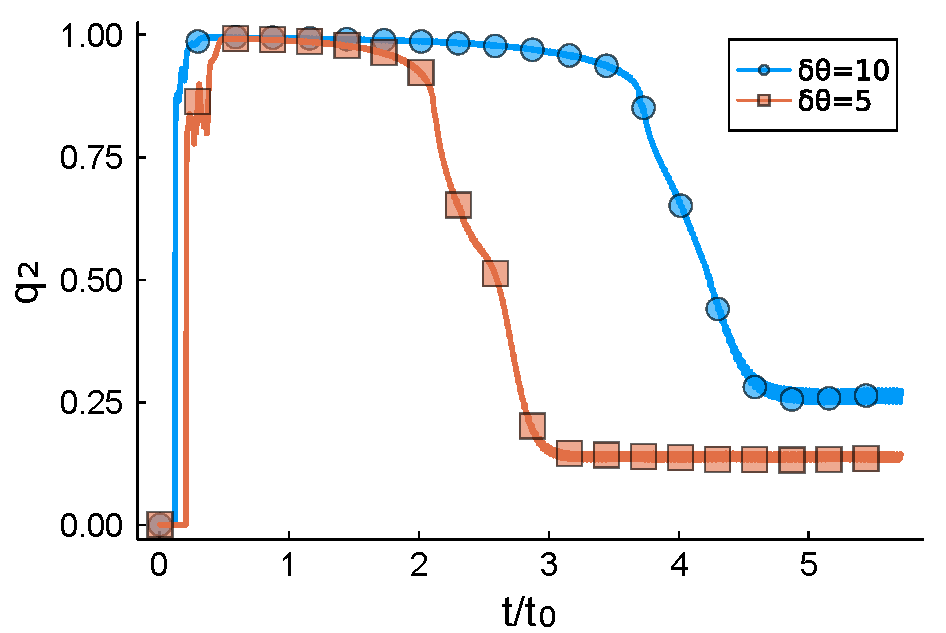
\includegraphics[width=0.75\textwidth]{gamma15_deltaTheta.pdf}
    \caption{Comparison of the Minkowski's structure metric $q_2$ for 
    $\delta\theta = 5^{\circ}, 10^{\circ}$, 
    $\Gamma = 15$ and $\lambda = 256 h_0$.}
    \label{fig:dif_contrast}
\end{figure}
The rivulets lifetime, though, is shorter than the one for $\delta \theta = 10^{\circ}$.
We acknowledge, then, that a systematic study of the quantitative dependence of 
lifetimes on the full parameter space would be important, but we also that such a study
would deseve a dedicated, extended, work that goes somehow beyond the goal of the present paper and of a typical PRL contribution.
We have added the new figure and the relative discussion on $\delta \theta$ in the
Supplementary Material.\\
We agree, also, that it is appropriate to add further details in the text, therefore we commented in the revised version on the choice of the checkerboard pattern saying that:\\
\\
\textcolor{red}{We decorate the substrate with a checkerboard pattern, a common choice that generalizes the broken homogeneity of the stripes to two 
directions~\cite{KarguptaLangmuir2003,Jalali2018,Nagayama2020,Das2020}.}

}

\item[ \textbf{\underline{Comment 3.}}]
{ 
Also unclear is how does the substrate patterning scale $2\pi/q_\theta$ compare with the scale of homogeneous dewetting $2\pi/q_0$.
I tried hard to understand whether the different cases of $\lambda$ discussed in the paper agree with $2\pi/q_0$ but I was unable to do so. 
}

\item[ \textbf{{Answer}}]
{
We apologize for having lacked thoroughness not providing the numerical 
value of $q_0$ (of which we reported the expression, though) to compare with the 
other characteristic scales. Plugging in the values of $\theta_0$,
$h_0$ and $h_{\ast}$ we get $q_0 \approx 0.09 h_0^{-1}$, whence 
$\lambda_0 = 2\pi/q_0 \approx 70 h_0$, which corresponds approximately to the shortest pattern wavelength considered. 
In fact, it is known that for a periodic chemical pattern to be effective in 
confining droplets over the more hydrophilic patches, the pattern wavelength should 
not be smaller than the spinodal length scale on the less wettable substrate
($\lambda_l \approx 50$ in our case) \cite{KarguptaJCP2002,KarguptaLangmuir2000,Nisato1999,Karim1998}.
We have added comments on this important point in the revised manuscript, when discussing the accessible ranges of pattern wavelength (see also the answer to the comment 5).
}

\item[ \textbf{\underline{Comment 4.}}]
{  
How would the film behave if the dynamics of the film were controlled primarily by spinodal dewetting and not by the contact-angle pattern?
At the same time, if the two characteristic lengthscales ($=$ that of the spinodal dewetting and that of the patterned substrate) are suitably synchronized, perhaps rivulets can be rendered permanent rather than transient? Or is the dewetting, once initiated, immanently irreversible even for a
time-dependent contact-angle pattern like the one studied in LM17723?
}

\item[ \textbf{{Answer}}]
{
The pattern-driven instability overwhelms the spinodal instability because it is active even on an initially flat film 
(i.e., where the initial perturbation $|\delta h_0| \rightarrow 0$) 
\cite{KonnurPRL2000,KarguptaLangmuir2000,KarguptaPRL2001}; ideally one would need to have a vanishing 
contact angle mismatch in order to see the spinodal dewetting, namely $\delta \theta \sim \delta h_0/h_0$,
which is also somehow obvious, but it would eventually deprive the pattern of meaning. 
The emergence of rivulets is observed even for $\lambda \approx \lambda_s$, as we show 
in Fig. \ref{fig:q2_difflambda}, but their nature is still metastable. 
\begin{figure}
    \centering
    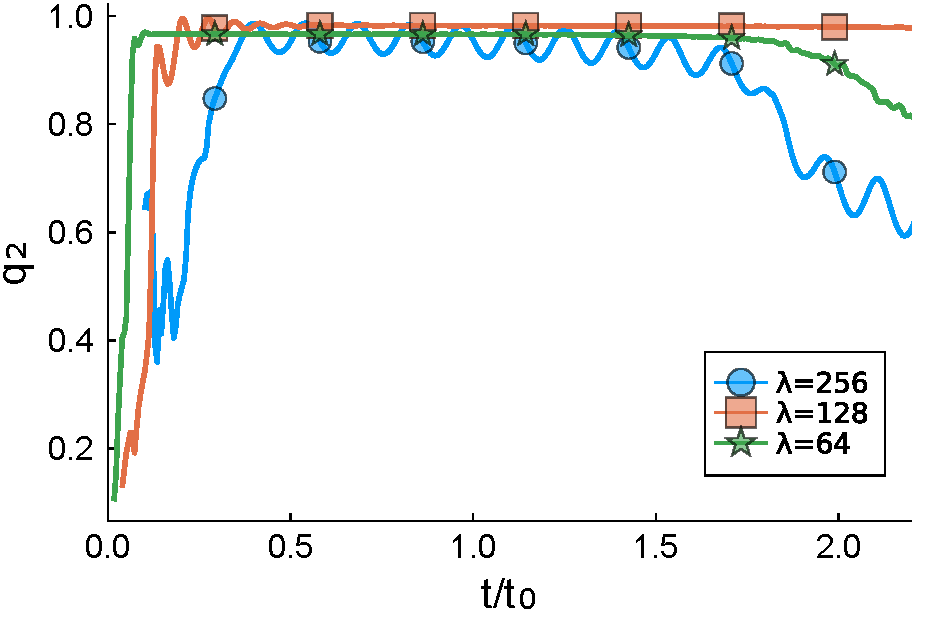
\includegraphics[width=0.8\textwidth]{lam_256-128-64-51.pdf}
    \caption{Minkowski's structure metric $q_2$ for three different wavelengths $\lambda=64 h_0$, $\lambda=128 h_0$ and $\lambda=256 h_0$ (as in figure 4 of the main text) and for $\Gamma=1.5$ (all other parameters are as in the main text). The time interval during which $q_2 \approx 1$ signals the emergence of rivulets, also for 
    $\lambda = 64 h_0$ which is comparable with the spinodal wavelength $\lambda_s \approx 70 h_0$}
    \label{fig:q2_difflambda}
\end{figure}
We have included also this new figure in the Supplementary Material.
}

\item[ \textbf{\underline{Comment 5.}}]
{ 
Many of the numerical results are supported by scaling estimates. I
like these arguments, but the agreement is hardly convincing. For
example, the linear and the square scaling laws in Fig. 2 each cover a
small range (much less than a tenfold variation) and so it is hard to
see whether they really apply. 
The same goes for the rivulet lifetime in Fig. 5 where the trend is OK but most likely a scaling law different from $\log(v_{\theta})$ would do as well in the range of $\tau_{riv}$ covered by the numerical data.
}

\item[ \textbf{{Answer}}]
{ 
We are well aware that the parameter ranges are not too wide, but 
of course our method (as any other) has to cope with limitations. 
For example, the range of achievable wavelengths is limited from below 
by the need to stay above the spinodal characteristic length (as explained in the answer to comment 3), and from above by the size of the system (i.e. by computing resources). As for the rivulet lifetimes, analogously, for reasons intrinsic to the stability of the numerical method, much higher pattern speeds cannot be reached 
(in particular one has to comply with the condition $\Gamma \ll 5 \times 10^2$). We have added the following
words of caution in the revised manuscript:\\
\\
\textcolor{red}{A few comments on the ranges are noteworthy at this point. The wavelengths are obviously limited from above by the size of the computational domain. On the other extreme, too short wavelengths are prevented by
the energetic cost of accomodating droplets on too
small patches, since the local contact angle (that increases with decreasing $\lambda$) would possibly exceed the largest substrate contact angle, such that the patterning 
itself would loose meaning. 
It has been, in fact, proven, both theoretically and experimentally, that 
for the confinement to be effective, the pattern characteristic size should 
not be much smaller than the spinodal length scale on the less wettable substrate
\cite{KarguptaJCP2002,KarguptaLangmuir2000,Nisato1999,Karim1998}.
We keep, therefore, $\lambda \stackrel{>}{\sim} \lambda_s \approx 70 h_0$. 
The pattern speeds, on the other hand, are limited by the intrinsic LB bound of the lattice speed of sound
 \cite{succi}.}\\
\\
We tend to disagree, instead, with the comment that any other scaling 
law would be equivalently good. Essentially because the logarithm scaling is 
not a fit, it is the result of a derivation based on plausible theoretical arguments, that 
is 'OK' with the numerical data.
%We think, anyhow, that the Referees' concerns are legitimate and we have, therefore, added 
%comments of caution about the scaling laws in the revised text.
Let us remark, though, that even in real microfluidic systems, 
one cannot expect too wild (and wide) variation of lengths and velocities.
In fact, we would be glad if our pioneering study might motivate further work 
in this direction, hopefully confirming our findings on an extended parameter 
range. Of course, that is more likely to happen if our message is conveyed
by a contribution in a high impact journal such as PRL. 
}

\end{itemize}

\bibliographystyle{abbrv}
\bibliography{Ref}

\end{document}
